\newpage
\section{Ocena operatorów BSP}

\subsection{Tradycyjna forma egzaminu}
\label{sec:tradycyjny-egzamin}
W niniejszej pracy, system stosowany jest jako narzędzie pomocnicze w przygotowaniu kandydatów do egzaminu praktycznego w celu uzyskania Świadectwa Kwalifikacji Presonelu Lotniczego z uprawnieniem podstawowym UAVO. Obecnie, egzamin praktyczny jest wymagany jedynie dla operatorów planujących loty w kategorii szczególnej\cite{ulc2019}, natomiast ogólne zasady lotu i kompetencje pozostają podobne. Ponadto uwarunkowania epidemiologiczne panujące od wprowadzenia nowych przepisów z końcem roku 2020 do momentu pisania niniejszej pracy, powodują trudności w organizacji egzaminów praktycznych. Z tych powodów, zadania będą przygotowywane dla egzaminów prowadzonych na podstawie wycofanych przepisów krajowych, a nie obowiązujących przepisów europejskich. Znaczna większość operacji BSP odbywa się na wielowirnikowcach --- dawna kategoria UAVO(MR), obecnie NSTS-02 oraz NSTS-06. Z tego powodu w następujących rozważaniach będzie uwzględniony tylko ten typ statku powietrznego.

Egzamin praktyczny do uzyskania na uprawnień operatora BSP składa się z kilku etapów, obejmujących także przygotowanie do lotu oraz obsługę naziemną\cite{ulc2014}. Przygotowywany system oceny dotyczy tylko jakości pilotażu, do których odnoszą się zadania w zakresie ,,Wykonywanie czynności lotniczych''. Znajomość postępowania w sytuacjach awaryjnych jest weryfikowana tylko przez omówienie, więc także zostanie pominięta.

Zasady egzaminu praktycznego nie zawierają konkretnych wartości tolerancji dla poszczególnych parametrów lotu. Zadaniem egzaminatora Lotniczej Komisji Egzaminacyjnej jest uznanie czy zaprezentowany poziom umiejętności jest wystarczający do bezpiecznego prowadzenia lotów BSP. Wśród wyszczególnionych kryteriów niezaliczenia egzaminu praktycznego, stosowane są zwroty odnoszące się do ,,utraty kontroli nad statkiem powietrznym'', ,,braku umiejętności pilotażu'', oraz ,,zagrożenia bezpieczeństwa''. Takie przedstawienie warunków zaliczenia umożliwia egzaminatorowi dostosowanie wymagań do osiągów statku powietrznego na którym przeprowadzany jest egzamin, rodzaju uzyskiwanych uprawnień oraz panujących warunków meteorologicznych. Z braku bardziej precyzyjnych źródeł pisemnych, opis wymogów dla poszczególnych zadań w tabeli \ref{tab:ocena-egzamin} jest oparty o własne doświadczenia autora pracy\footnote{Uzyskanie uprawnienia podstawowego UAVO VLOS (operacje w zasięgu wzroku); uzyskanie uprawnień dodatkowych BVLOS(operacje poza zasięgiem wzroku), MR 25 kg, A 25 kg (odpowiednio loty wielowirnikowymi i stałopłatami BSP o maksymalnej masie startowej do 25 kg); ukończenie szkolenia do uzyskania uprawnienia dodatkowego INS (instruktor)}. Zadanie zawisu dotyczy tylko bezzałogowych statków powietrznych pionowego startu i lądowania, a skoro analizowany jest przypadek wielowirnikowca zostało także ujęte w zestawieniu.

Zawis obowiązkowo wykonywany jest w różnych orientacjach, z przodem BSP skierowanym ,,we wszystkich kierunkach'', co w praktyce realizowane jest w następujących konfiguracjach:
\begin{itemize}
    \item tyłem BSP w kierunku do operatora
    \item prawą burtą do operatora
    \item przodem do operatora
    \item lewą burtą do operatora
\end{itemize}
Ma to na celu sprawdzenie umiejętności sterowania kiedy kierunki określone względem osoby pilotującej nie pokrywają się z kierunkami w których działają sterownice. Warto podkreślić że to zagadnienie nie występuje w lotnictwie załogowym, w którym pilot stale zajmuje pozycję skierowany do przodu statku powietrznego. Często lot po prostej także jest wykonywany w cztery różne strony, aby zweryfikować tę samą umiejętność w ruchu.

\begin{table}[!h] \centering
    \caption{Zestawienie zadań z elementami ocenianymi przez egzaminatora}
    \label{tab:ocena-egzamin}

    \begin{tabular}{| l *{8}{| c} |}
    \hline
    \textbf{Oceniane parametry} &
    \spheading{Wykonywanie startu} &
    \spheading{Utrzymanie równowagi w locie po prostej} &
    \spheading{Wprowadzanie i wyprowadzanie z zakrętu, krążenie} &
    \spheading{Zmiana wysokości lotu} &
    \spheading{Wykonywanie lądowania w wyznaczony obszar} &
    \spheading{Zawis \\ (w przypadku VTOL)} \\ \hline \hline
    \parbox{15em}{\raggedright Utrzymanie bezpiecznej odległości od osób i przeszkód}
                                 & \tick & \tick & \tick & \tick & \tick & \tick \\ \hline
    Poprawka na wiatr            & \tick & \tick & \tick &       & \tick & \tick \\ \hline
    Przód BSP w kierunku ruchu   &       & \tick & \tick &       &       &       \\ \hline
    Przód BSP w zadanym kierunku &       &       &       &       &       & \tick \\ \hline
    Utrzymanie stałej wysokości  &       & \tick & \tick &       &       & \tick \\ \hline
    Utrzymanie stałej prędkości  &       & \tick & \tick &       &       &       \\ \hline
    Utrzymanie zadanej pozycji   &       &       &       &       & \tick & \tick \\ \hline
    \parbox{15em}{\raggedright Przyziemienie z bezpieczną prędkością opadania}
                                 &       &       &       &       & \tick &       \\ \hline
  \end{tabular}
\end{table}

Parametry lotu zebrane w tabeli \ref{tab:ocena-egzamin} mogą być sugestią dla egzaminatora, oraz celem do którego dążą instruktorzy w trakcie szkolenia. Opis subiektywnej interpretacji terminu ,,utrzymanie kontroli nad statkiem powietrznym'' najłatwiej oprzeć na przykładach. Najczęściej wystąpienie pewnej niewielkiej odchyłki od wzorca nie powoduje zakończenia egzaminu z wynikiem negatywnym. Na przykładzie wykonywania zawisu, kiedy wskutek zmiennego wiatru BSP przemieścił się o jeden metr na stronę zawietrzną, operator powinien zareagować poprzez odpowiednie wychylenie drążka pochylenia i przechylenia aby powrócić do pierwotnie zadanej pozycji. Jeśli według instruktora odchyłka była adekwatna do panujących warunków i osiągów BSP, a reakcja wykonana poprawnie z zadowalająco małym opóźnieniem, można kontynuować zadanie. Natomiast wykonanie ruchu sterownicami który pogłębia uchyb sterowania można interpretować jako dowód braku umiejętności pilotażu, a w efekcie ostrzeżenie lub przerwanie zadania. Podobnie, stały niewielki błąd utrzymywania pozycji przez cały okres zawisu nie musi być podstawą do niezaliczenia próby, ale nawet krótkie niebezpieczne zbliżenie do człowieka powoduje nieukończenie egzaminu.

Próba zaprogramowania wszystkich niuansów oceny w celu zastąpienia egzaminatora lub instruktora byłaby wyjątkowo trudna, jeśli w ogóle możliwa. Zarówno w lotnictwie załogowym i bezzałogowym, ponad automatycznymi systemami pracuje człowiek weryfikujący poprawne działanie. Ostateczna ocena poziomu ryzyka oraz odpowiedzialność za bezpieczeństwo należą do odpowiednio przygotowanego personelu. Z tego powodu proponowana ocena liczbowa może pełnić jedynie funkcję pomocniczą. Można ją traktować jako kolejne źródło informacji, obok obserwacji wzrokowej i dialogu z operatorem.

\subsection{Wstęp do optymalizacji sterowania}
\label{sec:ocena-teoria}
Statek powietrzny wraz ze swoim operatorem można zamodelować jako układ ze sprzężeniem zwrotnym, w którym sterujący lotem człowiek jest regulatorem---jedynym, jak na rysunku \ref{fig:modelpilota}, lub jednym z wielu. Ponieważ w eksploatacji załogowych statków powietrznych, szczególnie śmigłowców, wpływ reakcji pilota ma duże znaczenie dla bezpieczeństwa i stabilności pewnych stanów lotu, modele tego typu są szczegółowo zbadane w literaturze\cite{roskam1998}. Taka reprezentacja interfejsu człowiek-maszyna sugeruje możliwość zastosowania narzędzi matematycznych opracowanych w celu oceny automatycznych układów regulacji do oceny sterowania wykonywanego przez operatora.

\begin{figure}[!h]
    \centering 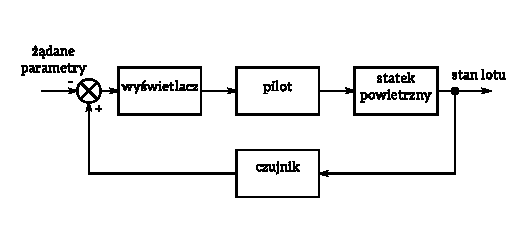
\includegraphics[width=0.8\linewidth]{modelpilota.pdf}
    \caption{Przedstawienie pilota jako regulatora dla statku powietrznego}
    \label{fig:modelpilota}
\end{figure}

Problem optymalizacji sterowania można opisać matematyczne jako minimalizację odpowiednio zdefiniowanej wielkości zwanej ,,kosztem'', która ma tym mniejszą wartość, im lepsza jest jakość sterowania. W ogólnym przypadku, zapis przypadków dla różnych sterowników może przyjąć formę funkcjonału z równania \ref{eq:pontryagin} \cite{ross2009}. Został podzielony na koszt końcowy\footnote{ang. \emph{endpoint cost}} oraz koszt bieżący\footnote{ang. \emph{running cost}}. Drugi z nich w ogólnej postaci jest całką w czasie odpowiedniej funkcji $ F $ zależnej od stanu obiektu $ x $ oraz sterowania $ u $. Ponieważ w przypadku lotu BSP oceniany jest proces trwający w czasie, dużo większe znaczenie przypisano do określenia kosztu bieżącego.

\begin{align}
    \label{eq:pontryagin}
    J[\vec{x}(\cdot), \vec{u}(\cdot), t_0, t_k] :=E\,[\,\vec{x}(t_0),t_0,\vec{x}(t_k),t_k\,] + \int\limits_{t_0}^{t_k} F\,[\,\vec{x}(t),\vec{u}(t),t\,] \,\operatorname{d}t
\end{align}

W literaturze na temat sterowania optymalnego wykorzystywane są różne liczbowe wskaźniki jakości regulacji, których sensem jest premiowanie pożądanych właściwości układu. W tabeli \ref{tab:wskazniki} zebrano niektóre ze stosowanych kryteriów, oraz interpretację ich wartości w kontekście oceny właściwości regulatora\cite{tan2004}, \cite{kaczorek2015}. Warto zwrócić uwagę, że wszystkie funkcje które są całkowane w poniższych wzorach są nieujemne pod warunkiem że stan modelu i sterowania należą do zbioru liczb rzeczywistych, co jest zawsze spełnione w opracowywanym systemie. Sprawia to, że w miarę upływu czasu miara jakości regulacji może jedynie narastać lub pozostawać na stałym poziomie. Ta wspólna własność powoduje, że oprócz opisanych poniżej kryteriów premiowana jest szybkość regulacji. O ile krótki czas działania jest niemal uniwersalnie pożądany wśród regulatorów układów automatycznych, zadania stawiane przed operatorem BSP mogą wymagać jedynie odpowiedniej precyzji bez przywiązywania dużej uwagi do szybkości wykonania. W tych przypadkach wyniki całkowania zostaną podzielone przez długość odcinka czasu w którym prowadzono ocenę. Zgodnie z definicją, otrzymana w ten sposób wartość będzie średnią całkową w czasie danej funkcji.

\begin{table}[!h] \centering
    \caption{Zestawienie wybranych wskaźników jakości regulacji}
    \label{tab:wskazniki}
    \renewcommand{\arraystretch}{1.3} % Wyższe o 30% rzędy tabeli

    \begin{tabular} {| l | l |} \hline
        \textbf{Definicja wielkości} & \textbf{Nazwa} \\ \hline\hline
        $ x(t) $ & stan układu \\ \hline
        $ u(t) $ & sterowanie układu \\ \hline
        $ r(t) $ & wartość zadana \\ \hline
        $ e(t) = r(t) - x(t) $ & uchyb \\ \hline\hline
        \textbf{Definicja wskaźnika} & \textbf{Interpretacja zastosowania} \\ \hline\hline
        $ \int_{t_0}^{t_k}{|e| \operatorname{d}t} $ & \multirow{4}*{minimalizacja błędu} \\ \cline{1-1}
        $ \int_{t_0}^{t_k}{e^2 \operatorname{d}t} $ & \\ \cline{1-1}
        $ \int_{t_0}^{t_k}{t \cdot |e| \operatorname{d}t} $ & \\ \cline{1-1}
        $ \int_{t_0}^{t_k}{t \cdot e^2 \operatorname{d}t} $ & \\ \hline
        $ \int_{t_0}^{t_k}{1 \operatorname{d}t} $ & minimalizacja czasu regulacji\\ \hline
        $ \int_{t_0}^{t_k}{u^2 \operatorname{d}t} $ & minimalizacja energii sterowania \\ \hline
    \end{tabular}
\end{table}

Duża część funkcji opisanych w tabeli jest przeznaczona do zastosowania dla układu o jednym stopniu swobody, w którym uchyb jest wielkością skalarną. W przypadku oceny różnych parametrów lotu, konieczne staje się łączenie kilku wskaźników obliczonych na podstawie różnych wielkości. Aby zapewnić łatwość interpretacji wyników, zbiorcza ocena jest obliczana jako kombinacja liniowa poszczególnych wskaźników jakości sterowania. Współczynniki poszczególnych składników mają realizować jednocześnie zadanie normalizacji wartości do zbliżonego przedziału wartości, a także umożliwiać dostosowywanie wpływu poszczególnych błędów na ogólną ocenę.

\subsection{Dobór kryteriów liczbowych}
W laboratorium symulatorów Wydziału Mechanicznego Energetyki i Lotnictwa, przed realizacją niniejszej pracy prowadzone były różne badania na temat wpływu czynnika ludzkiego na pilotaż statków powietrznych oraz prowadzenie innych pojazdów mechanicznych\cite{kopyt2017},\cite{kopyt2019}. Tematem jednej z prac dyplomowych opracowanych w laboratorium\cite{tomaszewska2019} jest algorytm do obiektywnej oceny komfortu pasażerów podczas podróży środkiem transportu, uwzględniając ze szczególną uwagą parametry lotu śmigłowca. Podobnie jak w niniejszej pracy, celem badań było opracowanie i ocena jakości liczbowego kryterium które może zastąpić subiektywną ocenę przebiegu danego zjawiska. Mimo tego, pewne cechy algorytmu opracowanego we wspomnianej pracy sprawiły że zdecydowano o utworzeniu innych kryteriów oceny.

Opracowywany w niniejszej pracy system umożliwia użytkownikowi zastosowanie dowolnego kryterium oceny, pod warunkiem że korzysta z  danych wysyłanych z aplikacji graficznej oraz jest możliwe do implementacji w wybranym przez siebie środowisku programowania. Przykładowo dla oceny jakości sterowania szybowcem, można oprzeć ocenę na wysokości lotu, lub po odpowiedniej modyfikacji aplikacji (por. \ref{sec:komunikacja}), na przykład o wartość prądu elektrycznego pobieranego przez zespół napędowy.

Egzamin praktyczny nie ma przypisanej skali ocen, a zaledwie jeden z dwóch rezultatów --- pozytywny lub negatywny. Symboliczna interpretacja kryteriów egzaminu w postaci określonej w równaniu \ref{eq:pontryagin} mogłaby wyglądać w sposób przedstawiony we wzorze \ref{eq:egzamin}, gdzie wartości logiczne $ A $, $ B $, etc. oznaczają wystąpienie danego typu zdarzenia niebezpiecznego lub wskazującego na utratę sterowania.
\begin{align}
    \label{eq:egzamin}
    E\left( \vec{x}(t) \right) &=
    \left\{
        \begin{array}{ll}
            \infty \mbox{ jeżeli } A \lor B \lor C \dots \\
            0 \mbox{ jeżeli } \neg ( A \lor B \lor C \dots)
        \end{array}
    \right.
    \\
    F & \equiv 0
\end{align}

Aby opracowany system był użyteczny do szkolenia, oraz umożliwiał porównanie umiejętności pomiędzy poszczególnymi operatorami, konieczne jest wprowadzenie większej rozdzielczości oceny niż tylko dwa skrajnie różne wyniki. Mimo to, pożądane jest aby zastosowana metryka chociaż częściowo oddawała charakter oceniania na egzaminie. Podobną, choć bardziej umiarkowaną charakterystykę mocnego penalizowania dużych odchyłek można osiągnąć stosując całkę z kwadratu błędu. W przypadku pewnych jednorazowych zdarzeń, jak na przykład kolizja z przeszkodą, egzamin praktyczny byłby przerwany. Także w tym obszarze wprowadza się bardziej stopniowaną ocenę, do każdego typu zdarzenia $ i $ przypisując wartość kary $ k $. Dzięki temu, w przypadku zadań wyjątkowo trudnych pod tym względem, można nadal porównywać podejścia między sobą na podstawie liczby wystąpienia zdarzeń, oznaczonej $ n $. Postać takiej funkcji kosztu oceniającej na podstawie $ K $ typów zdarzeń oraz $ L $ parametrów lotu została przedstawiona we wzorze \ref{eq:rozdzielczosc}. Wartości $ l $ to wspomniane w podrozdziale \ref{sec:ocena-teoria} wagi poszczególnych parametrów.
\begin{align}
    \label{eq:rozdzielczosc}
    E[ \vec{x}(t) ] &= \sum_{i=1}^{K} k_i \cdot n_i
    \\
    F[ \vec{x}(t) ] &= \sum_{j=1}^{L} l_j \cdot \int_{t_0}^{t_k} [ x_j(t) - x_{ref_j}(t) ]^2 \operatorname{d}t
\end{align}

\begin{todo}
    Wzory są nie do końca jasne; opisać na rzutach na płaszczyźnie lub wykresie 2D.
\end{todo}
Spośród zadań części praktycznej zebranych w tabeli \ref{tab:ocena-egzamin}, do szczegółowej oceny liczbowej wybrano te które mają oceniane kilka parametrów oraz nie polegają na interakcji z podłożem. Ćwiczenia które spełniają te warunki to lot po prostej, lot w zakręcie oraz zawis. Mozna dla nich sformułować uchyb jako odległość $ \delta_{A,B} $ pomiędzy pozycją BSP $ P $ a pewną wzorcową krzywą $ s_{ref} $ opisującą trasę przelotu, lub punktem $ P_{ref} $ w przypadku zawisu. Analogicznie, wymogi dla sterowania kierunkowego w zadaniach związanych z ruchem można opisać jako minimalizację kąta pomiędzy kierunkiem przednim ramy BSP oraz kątem drogi $ \psi_{KD} $. W powietrzu nieruchomym względem podłoża, ten kąt byłby równy kątowi ślizgu. Dla zawisu jest oceniana minimalizacja różnicy pomiędzy kątem odchylenia BSP $ \psi $, a zadanym przez egzaminatora kierunkiem $ \psi_{ref} $. Rysunek \ref{fig:definicjebledu} zawiera graficzne przedstawienie wprowadzonych tu definicji. Zawis wykonywany jest przez określony, stały odcinek czasu. Aby większa długość wykonywania lotu po prostej nie wpływała negatywnie na wskaźnik oceny, wyniki całkowania są dzielone przez czas wykonywania ćwiczenia. W przypadku prowadzenia BSP w zakręcie, ćwiczenie należy wykonywać w dość szybkim locie, dlatego wartość celowo nie jest uśredniana. Podsumowanie kryteriów dla zadań w typowej kolejności wykonywania ich w trakcie egzaminu przedstawiono w tabeli \ref{tab:ocena-funkcje}.

\begin{figure}[!h]
    \centering 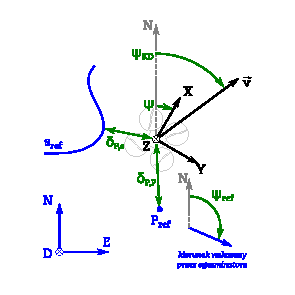
\includegraphics[width=0.8\linewidth]{definicjebledu.pdf}
    \caption{Szkic ilustrujący wielkości wykorzystywane w liczbowych wskażnikach oceny}
    \label{fig:definicjebledu}
\end{figure}

\begin{table}[!h] \centering
    \caption{Zestawienie zadań z funkcjami do ich oceny}
    \label{tab:ocena-funkcje}
    \renewcommand{\arraystretch}{1.3} % Wyższe o 30% rzędy tabeli

    \begin{tabular}{| l *{8}{| c} |}
    \hline
    \textbf{Oceniane parametry} &
    Zawis &
    \parbox{10em}{\raggedright Utrzymanie równowagi w~locie po prostej} &
    \parbox{10em}{\raggedright Wprowadzanie i~wyprowadzanie z~zakrętu, krążenie} \\ \hline \hline
    Ocena pozycji & $ \int{(\delta_{P,P_{ref}})^2 \operatorname{d}t} $ & $ \frac{1}{T} \int{(\delta_{P,s_{ref}})^2 \operatorname{d}t} $ & $ \int{(\delta_{P,s_{ref}})^2 \operatorname{d}t} $ \\ \hline
    Ocena kierunku & $ \int{(\psi - \psi_{ref})^2 \operatorname{d}t} $ & $ \frac{1}{T} \int{(\psi - \psi_{KD})^2 \operatorname{d}t} $ & $ \int{(\psi - \psi_{KD})^2 \operatorname{d}t} $ \\ \hline
    Czas wykonywania $ T $ & stały & bez wpływu na ocenę & nagradzany krótszy \\ \hline
  \end{tabular}
\end{table}

% \begin{todo}
%     Specjalnie zrobić przykładowe loty bardzo dobre i bardzo słabe żeby wskazać że te algorytmy oceny działają.
% \end{todo}